\section{Filastruder-sensor diámetro-bobinadora}
\label{sec:FSB}

Como primera aproximación e intentando asemejar el esquema de producción que tienen en la fábrica de Huesca se va a seguir el siguiente esquema:

\begin{figure}[H]
    \centering
    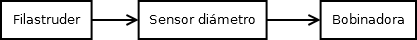
\includegraphics[width=0.6\textwidth]{images/producciones/Diagram1.png}
    \caption{Esquema de producción}
    \label{fig:esquemap_FSB}
\end{figure}

La boquilla de la filastruder es de 3mm, de esta manera tenemos margen suficiente para intentar regular el filamento aplicando una fuerza de tracción según sale de la extrusora y se va enfriando. A la hora de trabajar con una técnica de conformado como es esta, es muy importante que la velocidad de salida sea lo más constante posible y también hay que tener en cuenta que se producen cambios en el material tanto de tamaño como de forma según sale de la extrusora. Tres de estos cambios que afectan al material son: \cite{tecno_polimeros}

\begin{itemize}
	\item {\textbf{Tensionado}: Habitualmente, el material es recogido por sistemas de almacenamiento consistentes en rodillos que aplican una tensión. Esto hace que el tamaño del material varié en función de esa tensión. Nos ayudaremos de esta característica para intentar regular el diámetro final del filamento. El tamaño del diámetro tendrá una relación inversamente proporcional a la velocidad.}
	\item {\textbf{Relajación}: Dentro de la extrusora, el material soprta esfuerzos normales y  al salir por la boqquilla se relaja. Esta relajación será mayor, en función del gradiente de temperatura que haya entre la boquila y el ambiente.
		\begin{figure}[H]
	        \centering
	        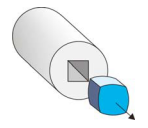
\includegraphics[width=0.2\textwidth]{images/producciones/relajacion.png}
	        \caption{Cambio de tamaño debido a la relajación del material. Fuente \cite{tecno_polimeros}}
	        \label{fig:prod_relajacion}
		\end{figure}
	}
	\item {\textbf{Enfriamiento}: A medida que el material se va enfriando, se va generando una contracción en el perfil del mismo. Está contraccion depende de la velocidad de enfriamiento del material. Por ello, no habrá la misma contracción en una zona gruesa donde haya más material, que en una fina.
		\begin{figure}[H]
	        \centering
	        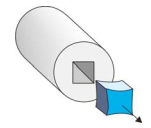
\includegraphics[width=0.2\textwidth]{images/producciones/contraccion.png}
	        \caption{Cambio de tamaño debido a la contraccion del material. Fuente \cite{tecno_polimeros}}
	        \label{fig:prod_contraccion}
		\end{figure}
	}
\end{itemize}

\subsection{Resultados}
Vamos a comprobar el funcionamiento del sistema con el control de regulación de la propia filawinder, en la que intenta mantener el filamento en una determinada altura y en función de esa altura, aplicar más o menos velocidad de bobinado. Para esta primera producción se usarán todos los pellets reciclados como materia prima, no se mezclará con PLA transparente, para así ver si el funcionamiento de la filastruder es el correcto.\\

Una vez llegado a la consigna de temperatura de 150ºC se comienza a extruir PLA reciclado y se almacena en la bobina. A simple vista, se ve que la velocidad mínima de bobinado hace que el filamento salga demasiado delgado y se generan demasiadas tensiones en el bobinado del mismo. No obstante, analizaremos los resultados obtenidos. Para el análisis del fihero CSV generado, se usará la herramienta ipython con las librerias, Numpy y Scypi, con los que de manera rápida obtendremos unas conclusiones.\\

Las condiciones iniciales del ensayo son:

	\begin{itemize}
		\item Hora de inicio: 11:50
		\item Hora de fin: 12:20
		\item Temperatura de extrusión: 150ºC
	\end{itemize}

Las medidas obtenidas en el ensayo son:

\begin{table}[H]
	\centering
	\begin{tabular}{ccc}
		{\bf } & {\bf Diámetro X} & {\bf Diámetro Y} \\ \hline
		Medidas & 1110.000000 & 1110.000000 \\
		Media (mm) & 1.17 & 0.91 \\
		Desviación estandar & 0.39 & 0.51 \\
		Mínimo (mm) & 0.01 & 0.00 \\
		Máximo (mm) & 1.92 & 1.74
	\end{tabular}
	\caption{Resultados obtenidos en la producción}
	\label{tab:result1}
\end{table}

Cómo podemos comprobar obtenemos una media aritmética de filamento de $ \bar{x} = 1.17mm $  mm con una desviación estandar  $\sigma = 0.39$. Representando las medidas de los ejes X e Y podemos comprobar que el resultado no es el deseado:

\begin{figure}[H]
	\centering
	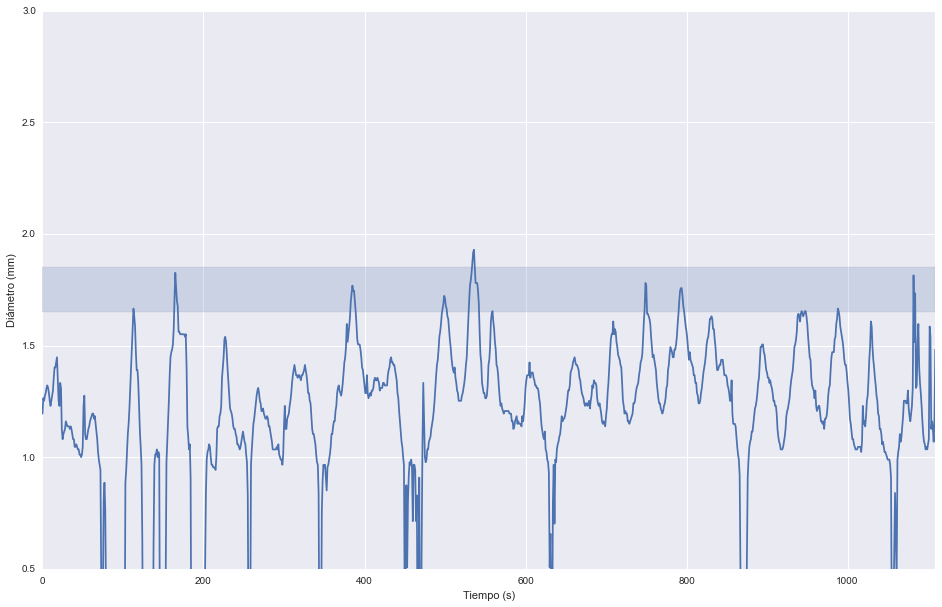
\includegraphics[width=0.8\textwidth]{images/producciones/16062015/output_9_1.png}
	\caption{Representación de las medidas de los ejes X e Y.}
	\label{fig:prod_ejes}
\end{figure}

Sólo un pequeño número de muestras están por dentro de los márgenes de calidad establecidos por BQ (Max = 1.85mm ; Min = 1.65mm). Además, si representamos los datos en un diagráma de cajas, vemos que hay mucha variación entre los dos ejes:
\begin{figure}[H]
    \centering
    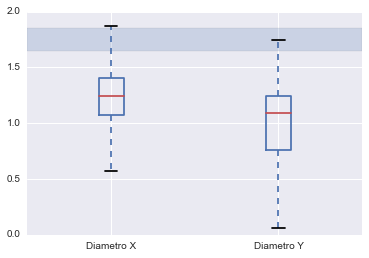
\includegraphics[width=0.5\textwidth]{images/producciones/16062015/output_10_1.png}
    \caption{Diagrama de cajas de las medidas de los ejes X e Y.}
    \label{fig:prod_boxplot}
\end{figure}

Después de los resultados obtenidos en el experimento, descartamos que con este esquema de producción y los materiales disponibles, lleguemos a regular el diámetro de salida de una forma çoptima, por tanto se trata de obtener otro esquema de producción para ganarantizar mejores resultados.